%!TeX spellcheck = en
\documentclass{beamer}
\usetheme[noptsans,navigation=true , FB=Informatik, frametotal=false]{TUKL}
\setbeamertemplate{navigation symbols}{}
\usepackage{xcolor}
\usepackage[english]{babel}
\usepackage[utf8]{inputenc}
\usepackage[ddmmyyyy]{datetime}
\usepackage{hyperref}
\usepackage{amssymb}
\usepackage{booktabs}
\usepackage{graphicx}
\usepackage{tikz}
\usetikzlibrary{arrows.meta, positioning}
% ===============================================
% IMAGES TO UPLOAD TO OVERLEAF (from plots/diagnostics/):
%   pr_curve.png, score_distributions.png, val_score_timelines.png
% (per_sensor_error.png optional -- referenced in a comment only)
% ===============================================
% A compact key-takeaway command (colored rule + bold line, fixed small size)
\newcommand{\takeaway}[1]{%
  \vspace{0.35em}\par\noindent\textcolor{blue!60!black}{\rule{\linewidth}{0.4pt}}\par
  \vspace{0.15em}{\small\textbf{Key Takeaway:} #1}}
% Robust image: shows the plot if present, else a clean placeholder (so the
% deck always compiles even before the PNGs are uploaded to Overleaf).
\newcommand{\plot}[2]{%
  \IfFileExists{#1}{\includegraphics[#2]{#1}}%
  {\fcolorbox{black!30}{black!5}{\parbox[c][0.42\textheight][c]{0.86\linewidth}{%
     \centering\small\textit{#1}\\[2pt]\scriptsize(upload this plot to Overleaf)}}}}
% ===============================================
\newcommand{\presentationDate}{13.07.2026}
\newcommand{\olatName}{\{Master-Project: Machine Learning 26\}}
\newcommand{\meetingTime}{14:00-15:30}
\newcommand{\meetingRoom}{36-336}
% ===============================================
\title{\vspace{0.5em}Unsupervised Anomaly Detection in Multivariate Sensor Time-Series}
\author{Group ML\_DL\_5 \\ Bhuvana Shikaripura Dasharatha \and Purna Chandra Nandigana}
\date[\presentationDate]{\includegraphics[width=0.5\textwidth]{logos/group-logo-text-new.png} \hspace{5em} \presentationDate}
\begin{document}
\maketitle

% ===================== SLIDE 2 =====================
\begin{frame}[shrink]{The Problem and the Constraint That Shaped Everything}
\begin{itemize}
\item \textbf{Task:} flag anomalous timesteps in an 18-sensor industrial distillation process (temperatures, pressures, flows)
\item \textbf{The hard constraint:} \emph{no anomaly labels on the training data}
\begin{itemize}\small
\item 28 train runs (unlabeled) $\;\vert\;$ 10 validation runs (labeled) $\;\vert\;$ 53 test runs (portal-scored)
\end{itemize}
\item \textbf{Consequence:} a supervised classifier is impossible -- there are no anomalies to learn from
\item \textbf{So we do novelty detection:} learn what \emph{normal} looks like, then flag whatever departs from it
\end{itemize}
\takeaway{No labels $\rightarrow$ we learn normal behaviour and measure deviation, not a normal-vs-anomaly boundary.}
\end{frame}

% ===================== SLIDE 3 =====================
\begin{frame}[shrink]{Our Approach in One Picture}
\begin{center}
\resizebox{!}{0.54\textheight}{%
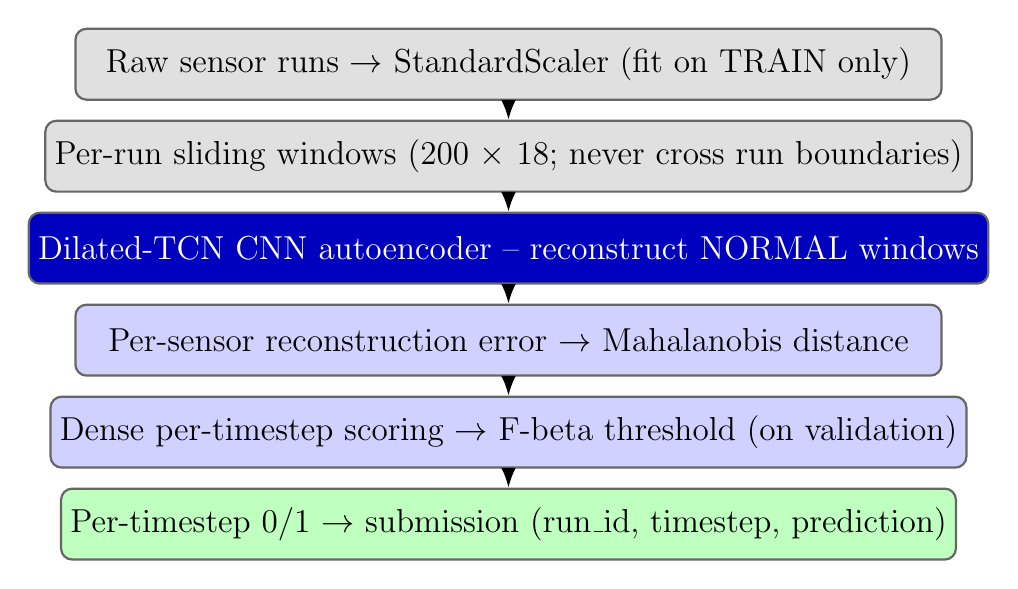
\begin{tikzpicture}[
  node distance=0.24cm,
  box/.style={rectangle, rounded corners, draw=black!60, thick,
              minimum width=11cm, minimum height=0.9cm, align=center, font=\large},
  greyBox/.style={box, fill=black!12},
  navyBox/.style={box, fill=blue!75!black, text=white},
  scoreBox/.style={box, fill=blue!18},
  outBox/.style={box, fill=green!25},
  arr/.style={-{Latex[length=2.5mm]}, thick}
]
\node[greyBox] (n1) {Raw sensor runs $\rightarrow$ StandardScaler (fit on TRAIN only)};
\node[greyBox, below=of n1] (n2) {Per-run sliding windows (200 $\times$ 18; never cross run boundaries)};
\node[navyBox, below=of n2] (n3) {Dilated-TCN CNN autoencoder -- reconstruct NORMAL windows};
\node[scoreBox, below=of n3] (n4) {Per-sensor reconstruction error $\rightarrow$ Mahalanobis distance};
\node[scoreBox, below=of n4] (n5) {Dense per-timestep scoring $\rightarrow$ F-beta threshold (on validation)};
\node[outBox, below=of n5] (n6) {Per-timestep 0/1 $\rightarrow$ submission (run\_id, timestep, prediction)};
\foreach \i/\j in {1/2,2/3,3/4,4/5,5/6} \draw[arr] (n\i) -- (n\j);
\end{tikzpicture}}
\end{center}
\takeaway{Learn normal $\rightarrow$ score surprise $\rightarrow$ threshold $\rightarrow$ predict. Labels touch only the checkpoint and threshold.}
\end{frame}

% ===================== SLIDE 4 =====================
\begin{frame}[shrink]{The Model: A Dilated-TCN Autoencoder}
\begin{columns}[T]
\begin{column}{0.50\textwidth}
\begin{center}
\resizebox{!}{0.60\textheight}{%
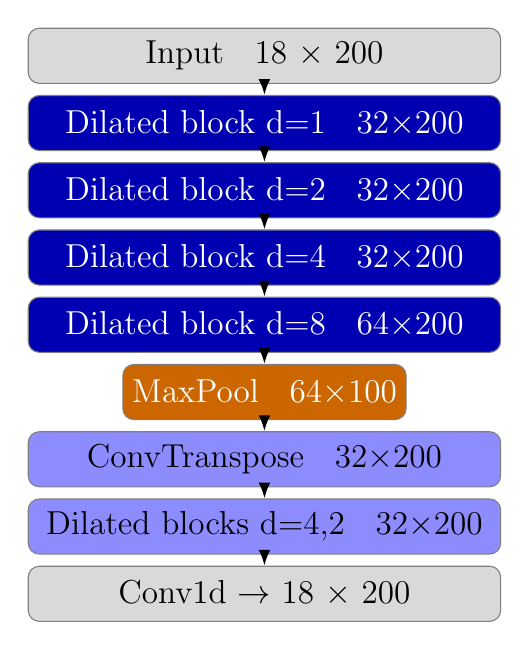
\begin{tikzpicture}[
  node distance=0.14cm,
  enc/.style={rectangle, rounded corners, draw=black!50, fill=blue!70!black, text=white, minimum height=0.7cm, align=center, font=\large},
  bot/.style={rectangle, rounded corners, draw=black!50, fill=orange!80!black, text=white, minimum height=0.7cm, align=center, font=\large},
  dec/.style={rectangle, rounded corners, draw=black!50, fill=blue!45, minimum height=0.7cm, align=center, font=\large},
  io/.style={rectangle, rounded corners, draw=black!50, fill=black!15, minimum height=0.7cm, align=center, font=\large},
  arr/.style={-{Latex[length=2mm]}, thick}
]
\node[io, minimum width=6cm] (a) {Input \; 18 $\times$ 200};
\node[enc, minimum width=6cm, below=of a] (b) {Dilated block d=1 \; 32$\times$200};
\node[enc, minimum width=6cm, below=of b] (c) {Dilated block d=2 \; 32$\times$200};
\node[enc, minimum width=6cm, below=of c] (d) {Dilated block d=4 \; 32$\times$200};
\node[enc, minimum width=6cm, below=of d] (e) {Dilated block d=8 \; 64$\times$200};
\node[bot, minimum width=3cm, below=of e] (f) {MaxPool \; 64$\times$100};
\node[dec, minimum width=6cm, below=of f] (g) {ConvTranspose \; 32$\times$200};
\node[dec, minimum width=6cm, below=of g] (h) {Dilated blocks d=4,2 \; 32$\times$200};
\node[io, minimum width=6cm, below=of h] (i) {Conv1d $\rightarrow$ 18 $\times$ 200};
\foreach \x/\y in {a/b,b/c,c/d,d/e,e/f,f/g,g/h,h/i} \draw[arr] (\x)--(\y);
\end{tikzpicture}}
\end{center}
\end{column}
\begin{column}{0.50\textwidth}
\small
\begin{itemize}
\item \textbf{Bottleneck} forces compression -- otherwise the AE just copies the input and reconstructs anomalies too
\item \textbf{Dilations 1,2,4,8} give a $\sim$63-step receptive field cheaply (the old conv saw only 3 steps)
\item \textbf{Why wide context?} the anomalies are slow drifts, not one-step spikes
\end{itemize}
\end{column}
\end{columns}
\takeaway{The bottleneck makes it good \emph{only} at normal; dilation lets it see the slow drifts.}
\end{frame}

% ===================== SLIDE 5 =====================
\begin{frame}[shrink]{The Key Idea: Per-Sensor Mahalanobis Scoring}
\small
\begin{itemize}
\item \textbf{Flat MSE fails:} a real spike on one precise sensor is averaged in with 17 sensors' noise -- diluted away
\item \textbf{Fix:} one error value per sensor (18-dim vector), then measure distance from the normal cloud:
\end{itemize}
\[
d^2 = (x-\mu)^{\top}\,\Sigma^{-1}\,(x-\mu)\qquad(\mu,\Sigma\ \text{via Ledoit--Wolf shrinkage on normal windows})
\]
\begin{itemize}\small
\item \textbf{Worked example (real val window):} FT703 spikes to $z=+5.99$ while T701 stays flat
\item error $\approx[\,0.04,\,4.8\,]\ \Rightarrow\ d^2\approx1058\ \gg\ $ threshold $\approx43\ \Rightarrow\ $\textbf{flagged (correct)}
\end{itemize}
\takeaway{Changing the \emph{scoring} -- with zero architecture change -- was the biggest single jump: F1 $0.48\rightarrow0.60$.}
\end{frame}

% ===================== SLIDE 6 =====================
\begin{frame}[shrink]{Thresholding and Evaluation}
\begin{columns}[c]
\begin{column}{0.52\textwidth}
\small
\begin{itemize}
\item A score must become 0/1: sweep the precision--recall curve on validation, pick the best cutoff
\item \textbf{Why F-beta, $\beta=0.5$?} distributions overlap, so plain F1 over-flagged 65--88\% of timesteps; $\beta<1$ weights precision
\item We also report \textbf{ROC-AUC} -- threshold-free ranking quality, the real ceiling
\end{itemize}
\end{column}
\begin{column}{0.48\textwidth}
\begin{center}
\plot{pr_curve.png}{height=0.50\textheight}
\end{center}
\end{column}
\end{columns}
\takeaway{$\beta=0.5$ curbs over-prediction; AUC -- not F1 -- tells us how good the model really is.}
\end{frame}

% ===================== SLIDE 7 =====================
\begin{frame}[shrink]{Results: The Full Journey}
\begin{center}
\footnotesize
\begin{tabular}{|l|c|c|}
\hline
\textbf{Stage} & \textbf{Val F1} & \textbf{ROC-AUC} \\
\hline
Phase 1--4: rebuilt code, fixed 6 correctness bugs & 0.41 & -- \\
Round 2: CNN checkpoint selection & 0.46 & -- \\
Round 3: dilated-TCN architecture & 0.48 & 0.65 \\
\textbf{Round 4: per-sensor Mahalanobis + F-beta} & \textbf{0.58--0.60} & \textbf{0.76} \\
Round 5: fusion tested \& rejected $\rightarrow$ CNN-only & 0.60 & 0.76 \\
\hline
\end{tabular}
\end{center}
\begin{itemize}\small
\item \textbf{Competition portal: F1 = 0.63} -- \emph{higher} than validation (0.60): not over-fit to the 10 val runs
\item The ROC-AUC jump ($0.65\rightarrow0.76$) is the meaningful part -- genuine separation, not a lucky threshold
\end{itemize}
\takeaway{Systematic, measured gains -- the Mahalanobis + F-beta round was the inflection point.}
\end{frame}

% ===================== SLIDE 8 =====================
\begin{frame}[shrink]{Why CNN-Only? We Tested Fusion Rigorously}
\begin{itemize}\small
\item \textbf{Hypothesis:} fuse the CNN with a \emph{diverse} tabular detector to cover blind spots
\item \textbf{Tested} Isolation Forest, then density-based LOF, with leakage-free run-grouped 5-fold CV choosing the weight
\end{itemize}
\begin{center}
\footnotesize
\begin{tabular}{|l|c|c|c|}
\hline
\textbf{Model (validation)} & \textbf{F1} & \textbf{ROC-AUC} & \textbf{Fusion weight} \\
\hline
CNN only & \textbf{0.59} & \textbf{0.77} & 1.00 \\
LOF only & 0.46--0.48 & 0.67 & -- \\
Hybrid (honest out-of-fold) & 0.55 & 0.72 & LOF 0.03 $\rightarrow$ 0.00 \\
\hline
\end{tabular}
\end{center}
\begin{itemize}\small
\item 9 of 10 folds chose \emph{pure CNN}; even a small LOF blend lowered F1 (more recall, worse precision)
\end{itemize}
\takeaway{Across three fusion attempts, no tabular detector beat the CNN -- CNN-alone is the honest, stronger choice.}
\end{frame}

% ===================== SLIDE 9 =====================
\begin{frame}[shrink]{We Looked Inside: The Score-Separability Ceiling}
\begin{columns}[c]
\begin{column}{0.55\textwidth}
\begin{center}
\plot{score_distributions.png}{height=0.50\textheight}
\end{center}
\end{column}
\begin{column}{0.45\textwidth}
\small
\begin{itemize}
\item Normal vs anomalous score histograms \textbf{overlap near zero} -- this overlap \emph{is} the ROC-AUC ceiling
\item The signal is carried mainly by flows and pressures (FT703, FT704, PDI702, T703)
\item No threshold breaks the overlap -- only a \emph{better score} raises F1
\end{itemize}
\end{column}
\end{columns}
\takeaway{The score overlap is the ceiling: raise the score, not the threshold.}
\end{frame}

% ===================== SLIDE 10 =====================
\begin{frame}[shrink]{A Diagnostic Discovery: The Global Threshold Breaks}
\begin{columns}[c]
\begin{column}{0.58\textwidth}
\begin{center}
\plot{val_score_timelines.png}{width=\linewidth}
\end{center}
\end{column}
\begin{column}{0.42\textwidth}
\small
\begin{itemize}
\item Raw score magnitudes vary $\sim$100$\times$ across runs
\item Two val runs score \textbf{F1 = 0} -- \emph{not} blindness: peaks sit on the anomalies but below the global threshold
\item \textbf{Fix:} per-run normalization (cheap, unsupervised)
\end{itemize}
\end{column}
\end{columns}
\takeaway{The within-run ranking is often correct -- a single global threshold is the next fixable bottleneck.}
\end{frame}

% ===================== SLIDE 11 =====================
\begin{frame}[shrink]{Where the Remaining F1 Is Lost}
\begin{itemize}\small
\item \textbf{Score-separability ceiling (the big one):} AUC $\sim$0.76 -- only a better score breaks the overlap
\item \textbf{Training-set contamination:} unlabeled ``normal'' data likely contains undetected anomalies
\item \textbf{Tuned on the same 10 runs:} window, architecture, checkpoint, threshold -- an optimistic estimate
\item \textbf{Threshold $\neq$ portal metric:} we optimise F0.5; the portal appears to grade F1 ($\sim$0.045 recoverable)
\item \textbf{Run-to-run variance:} identical configs scored 0.568--0.611 from stochasticity alone
\end{itemize}
\takeaway{The highest-leverage work raises AUC \emph{at the source}, not more threshold polishing.}
\end{frame}

% ===================== SLIDE 12 =====================
\begin{frame}[shrink]{Prioritised Roadmap (Grounded in 2024--26 Literature)}
\begin{enumerate}\small
\item \textbf{Contamination-robust training} -- down-weight likely-anomalous training windows (CLEANet / RiAD-style)
\item \textbf{Per-run score normalization} -- from our diagnostic; cheap, rescues the missed runs
\item \textbf{Seed-ensemble + fit Mahalanobis on train} -- variance reduction, better normal model
\item \textbf{Align threshold to the portal metric} -- near-free F1 if the portal grades F1
\item \textbf{Honest tuning split} -- reuse the run-grouped GroupKFold we already built
\end{enumerate}
\takeaway{Attack the dominant bottleneck (score quality) first, not the convenient one.}
\end{frame}

% ===================== SLIDE 13 =====================
\begin{frame}[shrink]{Summary}
\begin{itemize}\small
\item \textbf{What we built:} an unsupervised dilated-CNN autoencoder that learns normal 18-sensor behaviour and scores deviation via per-sensor Mahalanobis distance
\item \textbf{Result:} val F1 $0.494\rightarrow0.60$, ROC-AUC $\sim$0.65 $\rightarrow$ 0.76, \textbf{portal F1 = 0.63}
\item \textbf{Scientific rigour:} rejected fusion with leakage-free CV (an honest negative result) and diagnosed the exact failure modes
\item \textbf{Forward:} a clear, literature-grounded roadmap targeting the true bottleneck
\end{itemize}
\takeaway{A focused model we fully understand and validated honestly -- including its negatives -- with a concrete path forward.}
\end{frame}

\end{document}
